\chapter{Matrixalgebra}\label{chap:ch9}

I de foregående kapitler har vi set på begreber som lineære ligninger, echelonformer, rækkereduktion, lineær uafhængighed, vektorligninger og matrixligninger. For at løfte vores problemløsningsevner til næste niveau skal vi nu dykke ned i matrixalgebra. Matrixoperationer gør det muligt at håndtere komplekse systemer mere effektivt og bygger videre på det fundament, vi har lagt. Værktøjerne og teknikkerne i dette kapitel gør det lettere at arbejde med flere matricer og fører os frem mod dybere indsigt, herunder centrale idéer som sætningen om invertible matricer.

\section{Regning med matricer}
Regneoperationer på matricer som addition, subtraktion, skalering og multiplikation gør det muligt at kombinere og bearbejde matricer på enkle måder. Disse operationer er byggestenene i mere komplekse matrixmanipulationer, fx løsning af ligningssystemer og bestemmelse af inverse matricer.


\subsection*{Addition og multiplikation med skalar}
Vi begynder med definitionen af matrixaddition.

\begin{definition}{Matrixaddition}
    Lad $A$ og $B$ være $m \times n$-matricer. \textbf{Summen} af $A$ og $B$, betegnet $A + B$, er den $m \times n$-matrix, hvis indgange fås ved at addere de tilsvarende indgange i $A$ og $B$.

    For matricerne

    $$
    A=\left[\begin{array}{cccc}
    a_{11} & a_{12} & \cdots & a_{1 n} \\
    a_{21} & a_{22} & \cdots & a_{2 n} \\
    \vdots & \vdots & \vdots & \vdots \\
    a_{m 1} & a_{m 2} & \cdots & a_{m n}
    \end{array}\right], \quad B=\left[\begin{array}{cccc}
    b_{11} & b_{12} & \cdots & b_{1 n} \\
    b_{21} & b_{22} & \cdots & b_{2 n} \\
    \vdots & \vdots & \vdots & \vdots \\
    b_{m 1} & b_{m 2} & \cdots & b_{m n}
    \end{array}\right]
    $$

    som begge har dimensionen $m \times n$, er summen $A+B$ altså defineret som

    $$
    A+B=\left[\begin{array}{cccc}
    a_{11}+b_{11} & a_{12}+b_{12} & \cdots & a_{1 n}+b_{1 n} \\
    a_{21}+b_{21} & a_{22}+b_{22} & \cdots & a_{2 n}+b_{2 n} \\
    \vdots & \vdots & \vdots & \vdots \\
    a_{m 1}+b_{m 1} & a_{m 2}+b_{m 2} & \cdots & a_{m n}+b_{m n}
    \end{array}\right]
    $$
\end{definition}

\begin{remark}
    Tilsvarende gælder for subtraktion af matricer, selv om det ikke nævnes eksplicit her.
\end{remark}

Dernæst kommer definitionen af multiplikation af en matrix med en skalar. \newpage

\begin{definition}{Multiplikation med skalar}
    Lad $A$ være en $m \times n$-matrix og $c$ en skalar. \textbf{Produktet} af $c$ og $A$, betegnet $cA$, er den $m \times n$-matrix, hvis indgange fås ved at multiplicere hver indgang i $A$ med $c$. Produktet er altså defineret som

    $$
    c A=\left[\begin{array}{cccc}
    a_{11} & a_{12} & \cdots & a_{1 n} \\
    a_{21} & a_{22} & \cdots & a_{2 n} \\
    \vdots & \vdots & \vdots & \vdots \\
    a_{m 1} & a_{m 2} & \cdots & a_{m n}
    \end{array}\right] = \left[\begin{array}{cccc}
    c a_{11} & c a_{12} & \cdots & c a_{1 n} \\
    c a_{21} & c a_{22} & \cdots & c a_{2 n} \\
    \vdots & \vdots & \vdots & \vdots \\
    c a_{m 1} & c a_{m 2} & \cdots & c a_{m n}
    \end{array}\right]
    $$
    
\end{definition}

 \begin{example}
    Givet matricerne
    \[
A=\left[\begin{array}{ccc}
-5 & 2 & 0 \\
7 & -3 & 4 \\
-1 & 3 & 2
\end{array}\right] , \quad
B=\left[\begin{array}{ccc}
0 & -1 & 8 \\
6 & -14 & 2 \\
9 & 5 & 1
\end{array}\right]
\]
    skal du bestemme summen $A + B$ og produktet $3A$.
 \end{example}

\begin{solution}
    Summen $A + B$ fås ved at addere de tilsvarende indgange i $A$ og $B$:
\begin{align*}
\begin{split}
A+B & =\left[\begin{array}{ccc}
-5 & 2 & 0 \\
7 & -3 & 4 \\
-1 & 3 & 2
\end{array}\right]+\left[\begin{array}{ccc}
0 & -1 & 8 \\
6 & -14 & 2 \\
9 & 5 & 1
\end{array}\right] \\
& =\left[\begin{array}{ccc}
(-5)+(0) & (2)+(-1) & (0)+(8) \\
(7)+(6) & (-3)+(-14) & (4)+(2) \\
(-1)+(9) & (3)+(5) & (2)+(1)
\end{array}\right] \\
& =\left[\begin{array}{ccc}
-5 & 1 & 8 \\
13 & -17 & 6 \\
8 & 8 & 3
\end{array}\right]
\end{split}
\intertext{Produktet $3A$ fås ved at multiplicere hver indgang i $A$ med $3$:}
\begin{split}
3A & = 3 \left[\begin{array}{ccc}
-5 & 2 & 0 \\
7 & -3 & 4 \\
-1 & 3 & 2
\end{array}\right] \\
& = \left[\begin{array}{ccc}
3(-5) & 3(2) & 3(0) \\
3(7) & 3(-3) & 3(4) \\
3(-1) & 3(3) & 3(2)
\end{array}\right] \\
& = \left[\begin{array}{ccc}
-15 & 6 & 0 \\
21 & -9 & 12 \\
-3 & 9 & 6
\end{array}\right]
\end{split}
\end{align*}
\end{solution}

\begin{example}
Bestem $3A-2B$ for $A$ og $B$ nedenfor.
\[
    A=\left[\begin{array}{lll}
    1 & -2 & 5 \\
    0 & -3 & 9 \\
    4 & -6 & 7
    \end{array}\right], B=\left[\begin{array}{ccc}
    5 & 0 & -11 \\
    3 & -5 & 1 \\
    -1 & -9 & 0
    \end{array}\right]
    \]
    
\end{example}

\begin{solution}
    Vi beregner:

    \[
\begin{aligned}
3 A-2 B & =\left[\begin{array}{ccc}
3 & -6 & 15 \\
0 & -9 & 27 \\
12 & -18 & 21
\end{array}\right]-\left[\begin{array}{ccc}
10 & 0 & -22 \\
6 & -10 & 2 \\
-2 & -18 & 0
\end{array}\right] \\
& =\left[\begin{array}{ccc}
-7 & -6 & 37 \\
-6 & 1 & 25 \\
14 & 0 & 21
\end{array}\right]
\end{aligned}
\]
\end{solution}

Før vi går videre til matrixmultiplikation, skal vi formulere nogle grundlæggende algebraiske egenskaber ved matrixaddition og multiplikation med skalar.

\begin{theorem}

    Lad $A$, $B$, $C$ være matricer af samme størrelse, og lad $\alpha$, $\beta$ være skalarer. Så gælder
    \begin{enumerate}[(a)]
        \item $A+B=B+A$
        \item $(A+B)+C=A+(B+C)$
        \item $A+0=A$
        \item $\alpha(A+B)=\alpha A+\alpha B$
        \item $(\alpha+\beta) A=\alpha A+\beta A$
        \item $\alpha(\beta A)=(\alpha \beta) A$
    \end{enumerate}
\end{theorem}
\subsection*{Matrixmultiplikation}
Matrixmultiplikation er lidt mere kompliceret end addition og multiplikation med skalar. Produktet af to matricer er kun defineret, når antallet af søjler i den første matrix er lig med antallet af rækker i den anden matrix. Produktet af to matricer $A$ og $B$ er en ny matrix $C$, hvis indgange bestemmes af prikproduktet af rækkerne i $A$ og søjlerne i $B$. Bemærk, at $\vect{x}$ er en søjlevektor.

Lad \(B\) være en \(n \times p\)-matrix og \(A\) en \(m \times n\)-matrix. Hvis \(\vect{x} \in \mathbb{R}^p\), giver multiplikation af \(B\) med \(\vect{x}\) en ny vektor \(B\vect{x}\) i \(\mathbb{R}^n\). Når vi har dette resultat, kan vi multiplicere det videre med \(A\) og får \(A(B\vect{x})\), som er en vektor i \(\mathbb{R}^m\).

For enhver vektor \(\vect{x}\) i \(\mathbb{R}^p\) giver denne proces altså en tilsvarende vektor i \(\mathbb{R}^m\). Denne operation i to trin -- først multiplikation med \(B\) og derefter med \(A\) -- kaldes sammensætningen af \(A\) og \(B\) og skrives normalt som \(AB\). Vi har derfor:

\[
(AB)\vect{x} = A(B\vect{x})
\]

For at beregne den matrix, der fremkommer ved denne sammensætning, multiplicerer vi \(A\) direkte med \(B\) efter reglerne for matrixmultiplikation. Resultatet er en matrix \(C = AB\), hvor hver indgang i \(C\) bestemmes af samspillet mellem rækkerne i \(A\) og søjlerne i \(B\).

Grundlæggende er \(C\) den matrix, der udtrykker den samlede virkning af at anvende både \(B\) og \(A\) på en vilkårlig vektor \(\vect{x} \in \mathbb{R}^p\), uden at vi behøver at dele det op i mellemtrin.

\begin{definition}
    For $A \in \mathbb{R}^{m \times n}$ og $B \in \mathbb{R}^{n \times p}$, med $B=\left[\begin{array}{lll}\vect{b_1} & \vect{b_2} \cdots & \vect{b_p}\end{array}\right]$, definerer vi produktet $A B$ ved formlen

\[
A B=\left[\begin{array}{llll}
A \vect{b_1} & A \vect{b_2} & \cdots & A \vect{b_p}
\end{array}\right]
\]

\end{definition}

Produktet $AB$ er kun defineret, når antallet af søjler i $A$ er lig med antallet af rækker i $B$. Følgende diagram er nyttigt at huske det med:


\[
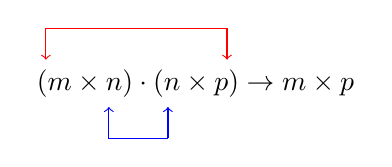
\begin{tikzpicture}
    % The matrix multiplication expression
    \node at (0,0) {\((m \times n) \cdot (n \times p) \rightarrow m \times p\)};
    
    % Red bidirectional U-shaped arrow on top
    \draw[red,<-] (-1.9,0.3) -- (-1.9,0.7) -- (0.4,0.7);
    \draw[red,->] (0.4,0.7) -- (0.4,0.3);
    
    % Blue bidirectional U-shaped arrow on the bottom
    \draw[blue,<-] (-1.1,-0.3) -- (-1.1,-0.7) -- (-0.35,-0.7);
    \draw[blue,->] (-0.35,-0.7) -- (-0.35,-0.3);
\end{tikzpicture}
\]

Diagrammet viser, at antallet af søjler i den første matrix skal være lig med antallet af rækker i den anden matrix (den \textcolor{blue}{blå pil}). Resultatet er en ny matrix med lige så mange rækker som den første matrix og lige så mange søjler som den anden matrix (den \textcolor{red}{røde pil}).

\begin{example}
    Beregn $AB$ og $BA$ for $A$ og $B$ nedenfor.

    \[
    A=\left[\begin{array}{lll}
    1 & 2 & -2 \\
    1 & 1 & -3
    \end{array}\right], \quad B=\left[\begin{array}{cccc}
    -4 & 2 & 4 & -4 \\
    -1 & -5 & -3 & 3 \\
    -4 & -4 & -3 & -1
    \end{array}\right]
    \]
    
\end{example}

\begin{solution}
    Først $A B=\left[\begin{array}{llll}A \vect{b_1} & A \vect{b_2} & A \vect{b_3} & A \vect{b_4}\end{array}\right]$:

\[
\begin{aligned}
& A B=\left[\begin{array}{lll}
1 & 2 & -2 \\
1 & 1 & -3
\end{array}\right]\left[\begin{array}{cccc}
-4 & 2 & 4 & -4 \\
-1 & -5 & -3 & 3 \\
-4 & -4 & -3 & -1
\end{array}\right] \\
& = \vcenter{\hbox{\begin{tikzpicture}
    \matrix (m1) [matrix of math nodes,left delimiter={[}] {
    2 & \quad \text{Række 1 i $A$ og søjle 1 i $B$} \\
    7 & \quad \text{Række 2 i $A$ og søjle 1 i $B$} \\
    };
    \draw[headercolor,thick] (m1-1-1.north west) rectangle (m1-2-1.south east);
\end{tikzpicture}}} \\
& = \vcenter{\hbox{\begin{tikzpicture}
    \matrix (m2) [matrix of math nodes,left delimiter={[}] {
    2 & 0 & \quad \text{Række 1 i $A$ og søjle 2 i $B$} \\
    7 & 9 & \quad \text{Række 2 i $A$ og søjle 2 i $B$} \\
    };
    \draw[headercolor,thick] (m2-1-2.north west) rectangle (m2-2-2.south east);
\end{tikzpicture}}} \\
& = \vcenter{\hbox{\begin{tikzpicture}
    \matrix (m3) [matrix of math nodes,left delimiter={[}] {
    2 & 0 & 4 & \quad \text{Række 1 i $A$ og søjle 3 i $B$} \\
    7 & 9 & 10 & \quad \text{Række 2 i $A$ og søjle 3 i $B$} \\
    };
    \draw[headercolor,thick] (m3-1-3.north west) rectangle (m3-2-3.south east);
\end{tikzpicture}}} \\
& = \vcenter{\hbox{\begin{tikzpicture}
    \matrix (m4) [matrix of math nodes,left delimiter={[}] {
    2 & 0 & 4 & 4 & \quad \text{Række 1 i $A$ og søjle 4 i $B$} \\
    7 & 9 & 10 & 2 & \quad \text{Række 2 i $A$ og søjle 4 i $B$} \\
    };
    \draw[headercolor,thick] (m4-1-4.north west) rectangle (m4-2-4.south east);
\end{tikzpicture}}} \\
& = \vcenter{\hbox{\begin{tikzpicture}
    \matrix (m4) [matrix of math nodes,left delimiter={[}, right delimiter={]}] {
    2 & 0 & 4 & 4 \\
    7 & 9 & 10 & 2 \\
    };
\end{tikzpicture}}}
\end{aligned}
\]

Derimod er $B A$ ikke defineret! $B$ har 4 søjler, og $A$ har 2 rækker. Antallet af søjler i $B$ er altså ikke lig med antallet af rækker i $A$. \end{solution}

\begin{example}
    Beregn matricen $A B$, hvor

\[
A=\left[\begin{array}{ll}
1 & 2 \\
2 & 3 \\
3 & 4
\end{array}\right], \quad \text { og } B=\left[\begin{array}{cc}
2 & -1 \\
3 & 1
\end{array}\right]
\]

\end{example}

\begin{solution}
    Ifølge definitionen af multiplikation ovenfor er

\[
\begin{aligned}
A B & =\left[A\left[\begin{array}{l}
2 \\
3
\end{array}\right] A\left[\begin{array}{c}
-1 \\
1
\end{array}\right]\right] \\
& \left.=\left[\begin{array}{ll}
1 & 2 \\
2 & 3 \\
3 & 4
\end{array}\right]\left[\begin{array}{l}
2 \\
3
\end{array}\right]\left[\begin{array}{ll}
1 & 2 \\
2 & 3 \\
3 & 4
\end{array}\right]\left[\begin{array}{c}
-1 \\
1
\end{array}\right]\right] \\
& =\left[\left[\begin{array}{l}
1 \cdot 2+2 \cdot 3 \\
2 \cdot 2+3 \cdot 3 \\
3 \cdot 2+4 \cdot 3
\end{array}\right]\left[\begin{array}{l}
1 \cdot(-1)+2 \cdot 1 \\
2 \cdot(-1)+3 \cdot 1 \\
3 \cdot(-1)+4 \cdot 1
\end{array}\right]\right] \\
& =\left[\begin{array}{cc}
8 & 1 \\
13 & 1 \\
18 & 1
\end{array}\right]
\end{aligned}
\]
\end{solution}

\begin{example} Hvis $A$ er $3 \times 5$ og $B$ er $5 \times 2$, hvilke størrelser har $A B$ og $B A$ så (forudsat at de er defineret)?
\end{example}

\begin{solution}
    \begin{itemize}
        \item Produktet $A B$ er defineret, da antallet af søjler i $A$ svarer til antallet af rækker i $B$ (5). Den resulterende matrix $A B$ er en $3 \times 2$-matrix.
        \item Produktet $B A$ er ikke defineret, da antallet af søjler i $B$ (2) ikke svarer til antallet af rækker i $A$ (3).
    \end{itemize}
\end{solution}

Det næste eksempel viser, at selv hvis både $AB$ og $BA$ er defineret, er de ikke nødvendigvis ens.

\begin{example}
    Beregn $AB$ og $BA$ for $A = \left[\begin{array}{rrr}
        -4 & 4 & 3 \\
        3 & -3 & -1 \\
        -2 & -1 & 1
        \end{array}\right] $ og $B = \left[\begin{array}{rrr}
            -1 & -1 & 0 \\
            -3 & 0 & -2 \\
            -2 & 1 & -2
            \end{array}\right]$.

\end{example}

\begin{solution}
    Først $AB$:

    \[
    \begin{aligned}
    A B &=\left[\begin{array}{rrr}
    -4 & 4 & 3 \\
    3 & -3 & -1 \\
    -2 & -1 & 1
    \end{array}\right]\left[\begin{array}{rrr}
    -1 & -1 & 0 \\
    -3 & 0 & -2 \\
    -2 & 1 & -2
    \end{array}\right] \\
    & =\left[\begin{array}{c}
    -14 \\
    8 \\
    3
    \end{array}\right. \\
    & =\left[\begin{array}{rr}
    -14 & 7 \\
    8 & -4 \\
    3 & 3
    \end{array}\right. \\
    & =\left[\begin{array}{rrr}
    -14 & 7 & -14 \\
    8 & -4 & 8 \\
    3 & 3 & 0
    \end{array}\right]
    \end{aligned}
    \]

    Dernæst $BA$:
    \[
    \begin{aligned}
    B A & =\left[\begin{array}{rrr}
    -1 & -1 & 0 \\
    -3 & 0 & -2 \\
    -2 & 1 & -2
    \end{array}\right]\left[\begin{array}{rrr}
    -4 & 4 & 3 \\
    3 & -3 & -1 \\
    -2 & -1 & 1
    \end{array}\right] \\
    & =\left[\begin{array}{rrr}
    1 \\
    16 & \\
    15
    \end{array}\right. \\
    & =\left[\begin{array}{rrr}
    1 & -1 \\
    16 & -10 \\
    15 & -9
    \end{array}\right. \\
    & =\left[\begin{array}{rrr}
    1 & -1 & -2 \\
    16 & -10 & -11 \\
    15 & -9 & -9
    \end{array}\right]
    \end{aligned}
    \]

    Vi ser, at $AB \neq BA$. \end{solution}

    I almindelig aritmetik er det neutrale element for multiplikation 1. I matrixalgebra er det neutrale element for multiplikation identitetsmatricen, som betegnes $I$. Identitetsmatricen er en \textit{kvadratisk} matrix med 1-taller i diagonalen og 0-taller alle andre steder. Identitetsmatricens størrelse bestemmes af sammenhængen og fremgår som regel klart af den. For eksempel er $I_2$ en $2 \times 2$-identitetsmatrix, og $I_3$ er en $3 \times 3$-identitetsmatrix, og generelt er $I_n \in \mathbb{R}^{n \times n}$ en $n \times n$-identitetsmatrix:

    $$
    I_n=\left[\begin{array}{ccccc}
    1 & 0 & 0 & \cdots & 0 \\
    0 & 1 & 0 & \cdots & 0 \\
    \vdots & \vdots & \vdots & \cdots & \vdots \\
    0 & 0 & 0 & \cdots & 1
    \end{array}\right]
    $$

    Vi kan nu formulere følgende sætning.

    \begin{theorem}
        Lad $A, B, C$ være matricer af passende dimensioner, og lad $\alpha$ være en skalar. Så gælder
\begin{enumerate}[(a)]
    \item $A(BC) = (AB)C$
    \item $A(B + C) = AB + AC$
    \item $(B + C)A = BA + CA$
    \item $\alpha(AB) = (\alpha A)B = A(\alpha B)$
    \item Hvis $A$ er en $m\times n$-matrix, så er $I_m A=A=AI_n$
\end{enumerate}
\end{theorem}

Vi afslutter dette afsnit med at se på den $k$'te potens af en matrix.

\begin{definition}
    Lad $A$ være en kvadratisk matrix, dvs. $ A \in \mathbb{R}^{n \times n}$. Den $k$'te potens af $A$, betegnet $A^k$, er defineret som produktet af $A$ med sig selv $k$ gange. Det vil sige

    $$
    A^k=\underbrace{ AAA \cdot \cdots A}_{k \text { gange }}
    $$

    hvor $A$ optræder $k$ gange på højre side.
\end{definition}

\begin{example}
    Beregn $A^3$, hvis
    \[
    A=\left[\begin{array}{rr}
    -2 & 3 \\
    1 & 0
    \end{array}\right]
    \]
\end{example}

\begin{solution}

    Beregn $A^2$:

    \[
    A^2=\left[\begin{array}{rr}
    -2 & 3 \\
    1 & 0
    \end{array}\right]\left[\begin{array}{rr}
    -2 & 3 \\
    1 & 0
    \end{array}\right]=\left[\begin{array}{rr}
    7 & -6 \\
    -2 & 3
    \end{array}\right]
    \]

    Og derefter $A^3$:

    \[
    \begin{aligned}
    A^3=A^2 A & =\left[\begin{array}{rr}
    7 & -6 \\
    -2 & 3
    \end{array}\right]\left[\begin{array}{rr}
    -2 & 3 \\
    1 & 0
    \end{array}\right] \\
    & =\left[\begin{array}{rr}
    -20 & 21 \\
    7 & -6
    \end{array}\right]
    \end{aligned}
    \]

    Vi kunne også gøre sådan:

    \[
    A^3=A A^2=\left[\begin{array}{rr}
    -2 & 3 \\
    1 & 0
    \end{array}\right]\left[\begin{array}{rr}
    7 & -6 \\
    -2 & 3
    \end{array}\right]=\left[\begin{array}{rr}
    -20 & 21 \\
    7 & -6
    \end{array}\right]
    \]

\end{solution}

\section{Den transponerede matrix}
Vi begynder med definitionen af den transponerede af en matrix.

\begin{definition}
    For en matrix $A \in \mathbb{R}^{m \times n}$ er den transponerede af $A$ matricen $A^T$, hvis $i$'te søjle er den $i$'te række i $A$.
\end{definition}

Hvis $A$ er $m \times n$, så er $A^T$ $n \times m$. Hvis for eksempel

\[
A=\left[\begin{array}{rrrrr}
0 & -1 & 8 & -7 & -4 \\
-4 & 6 & -10 & -9 & 6 \\
9 & 5 & -2 & -3 & 5 \\
-8 & 8 & 4 & 7 & 7
\end{array}\right]
\]

så er

\[
A^T=\left[\begin{array}{rrrr}
0 & -4 & 9 & -8 \\
-1 & 6 & 5 & 8 \\
8 & -10 & -2 & 4 \\
-7 & -9 & -3 & 7 \\
-4 & 6 & 5 & 7
\end{array}\right]
\]

\begin{example} Beregn $(AB)^T$ og $B^T A^T$, hvis

\[
A=\left[\begin{array}{rrr}
-2 & 1 & 0 \\
3 & -1 & -3
\end{array}\right], \quad B=\left[\begin{array}{rrr}
-2 & 1 & 2 \\
-1 & -2 & 0 \\
0 & 0 & -1
\end{array}\right].
\]
\end{example}

\begin{solution}
    Først beregner vi $(AB)^T$:

    \[
    \begin{aligned}
    A B &=\left[\begin{array}{rrr}
    -2 & 1 & 0 \\
    3 & -1 & -3
    \end{array}\right]\left[\begin{array}{rrr}
    -2 & 1 & 2 \\
    -1 & -2 & 0 \\
    0 & 0 & -1
    \end{array}\right] \\
    &=\left[\begin{array}{rrr}
        3 & -4 & -4 \\
        -5 & 5 & 9
        \end{array}\right]
    \end{aligned}
    \]

    og derefter $(AB)^T$:

    \[
    \begin{aligned}
    (A B)^{T} &=\left[\begin{array}{rrr}
        3 & -4 & -4 \\
        -5 & 5 & 9
        \end{array}\right]^{T} \\
    &=\left[\begin{array}{rr}
        3 & -5 \\
        -4 & 5 \\
        -4 & 9
        \end{array}\right]
    \end{aligned}
    \]

    Dernæst beregner vi $B^T A^T$:

    \[
    \begin{aligned}
    B^{T} A^{T} &=\left[\begin{array}{rrr}
        -2 & -1 & 0 \\
        1 & -2 & 0 \\
        2 & 0 & -1
        \end{array}\right]\left[\begin{array}{rr}
        -2 & 3 \\
        1 & -1 \\
        0 & -3
        \end{array}\right] \\
    &=\left[\begin{array}{rr}
    3 & -5 \\
    -4 & 5 \\
    -4 & 9
    \end{array}\right]
    \end{aligned}
    \]

    Vi ser, at $(AB)^T = B^T A^T$. \end{solution}

Følgende sætning opsummerer egenskaberne ved den transponerede af en matrix.

\begin{theorem}
    Lad $A$ og $B$ være matricer af passende dimensioner, og lad $\alpha$ være en skalar. Så gælder
    \begin{enumerate}[(a)]
        \item $(A^T)^T = A$
        \item $(A + B)^T = A^T + B^T$
        \item $(\alpha A)^T = \alpha A^T$
        \item $(AB)^T = B^T A^T$
    \end{enumerate}
\end{theorem}

En konsekvens af egenskab (4) er, at
\[
\left(A_1 A_2 \ldots A_k\right)^T=A_k^T A_{k-1}^T \cdots A_2^T A_1^T
\]

og som et specialtilfælde

\[
\left(A^k\right)^T=\left(A^T\right)^k
\]

\section{Invertible matricer}
Den inverse af en kvadratisk matrix \( A \in \mathbb{R}^{n \times n} \) udvider begrebet den reciprokke værdi af et reelt tal \( a \in \mathbb{R} \), der er forskelligt fra nul. Mere præcist er den inverse af et tal \( a \in \mathbb{R} \), der er forskelligt fra nul, det entydige tal \( c \in \mathbb{R} \), som opfylder \( a c = c a = 1 \). Den inverse af \( a \neq 0 \), som typisk skrives \( a^{-1} = \frac{1}{a} \), gør det muligt at løse ligningen \( a x = b \):

\[
a x = b \Rightarrow a^{-1} a x = a^{-1} b \Rightarrow x = a^{-1} b.
\]

Dette begreb kan udvides til kvadratiske matricer, hvor den inverse af en matrix \( A \in \mathbb{R}^{n \times n} \) er en matrix \( C \in \mathbb{R}^{n \times n} \), som opfylder \( A C = C A = I_n \), hvor \( I_n \) er identitetsmatricen af størrelse \( n \times n \). Den inverse af en matrix betegnes \( A^{-1} \). Vi kan nu definere en invertibel matrix.

\begin{definition}
    En kvadratisk matrix \( A \in \mathbb{R}^{n \times n} \) er invertibel (eller \textbf{ikke-singulær}), hvis der findes en matrix \( C \in \mathbb{R}^{n \times n} \), så \( A C = C A = I_n \). Matricen \( C \) kaldes den inverse af \( A \) og betegnes \( A^{-1} \). Der gælder altså \( A^{-1} A = A A^{-1} = I_n \).
\end{definition}

\begin{example}
    Vis, at $C$ er den inverse af $A$, hvor $A$ og $C$ er givet nedenfor.

    \[
    A=\left[\begin{array}{rrr}
    1 & -3 & 0 \\
    -1 & 2 & -2 \\
    -2 & 6 & 1
    \end{array}\right], \quad C=\left[\begin{array}{rrr}
    -14 & -3 & -6 \\
    -5 & -1 & -2 \\
    2 & 0 & 1
    \end{array}\right]
    \]
    \label{ex:inverse2}
\end{example}

\begin{solution}
    Vi skal vise, at $A C = C A = I_3$. Først beregner vi $AC$:

    \[
    \begin{aligned}
    A C &=\left[\begin{array}{rrr}
    1 & -3 & 0 \\
    -1 & 2 & -2 \\
    -2 & 6 & 1
    \end{array}\right]\left[\begin{array}{rrr}
    -14 & -3 & -6 \\
    -5 & -1 & -2 \\
    2 & 0 & 1
    \end{array}\right] \\
    &=\left[\begin{array}{rrr}
    1 & 0 & 0 \\
    0 & 1 & 0 \\
    0 & 0 & 1
    \end{array}\right]=I_3
    \end{aligned}
    \]

    Dernæst beregner vi $CA$:

    \[
    \begin{aligned}
    C A &=\left[\begin{array}{rrr}
    -14 & -3 & -6 \\
    -5 & -1 & -2 \\
    2 & 0 & 1
    \end{array}\right]\left[\begin{array}{rrr}
    1 & -3 & 0 \\
    -1 & 2 & -2 \\
    -2 & 6 & 1
    \end{array}\right] \\
    &=\left[\begin{array}{rrr}
    1 & 0 & 0 \\
    0 & 1 & 0 \\
    0 & 0 & 1
    \end{array}\right]=I_3
    \end{aligned}
    \]

    Vi ser, at $C=A^{-1}$ er den inverse af $A$. \end{solution}

Følgende sætning opsummerer sammenhængen mellem den inverse matrix og henholdsvis matrixmultiplikation og den transponerede matrix.

\begin{theorem} Lad $A$ og $B$ være invertible $n \times n$-matricer. Så gælder:
\begin{enumerate}[(a)]
    \item $A^{-1}$ er invertibel, og
    \[
    \left(A^{-1}\right)^{-1}=A
    \]
    \item Produktet $A B$ er invertibelt, og
    \[
    (A B)^{-1}=B^{-1} A^{-1}
    \]
    \item Den transponerede af $A$ er også invertibel, dvs. $A^T$ er invertibel, og
    \[
    \left(A^T\right)^{-1}=\left(A^{-1}\right)^T
    \]
\end{enumerate}

\end{theorem}

Vi ser nu på, hvordan vi kan bestemme den inverse af en matrix.

\subsection*{Bestemmelse af determinanten og den inverse af en $2 \times 2$-matrix}

Den inverse af en matrix er ikke altid let at bestemme. For en $2 \times 2$-matrix kan vi dog bruge en formel til at finde den inverse.

\begin{theorem}
    Lad $A=\left[\begin{array}{ll}
    a & b \\
    c & d
    \end{array}\right]$. Hvis $ad-bc \neq 0$, er den inverse af $A$ givet ved

    \[
    A^{-1}=\frac{1}{ad-bc}\left[\begin{array}{cc}
    d & -b \\
    -c & a
    \end{array}\right]
    \]
\end{theorem}

\begin{remark}
    Størrelsen $ad - bc$ kaldes determinanten af $A$, og vi skriver
    \[
    \text{det}(A) = |A| = ad - bc
    \]
\end{remark}

Determinanten af en $2 \times 2$-matrix er en skalar størrelse, der giver information om matricen. Hvis determinanten er nul, er matricen ikke invertibel. Hvis determinanten er forskellig fra nul, er matricen invertibel. De eksplicitte formler $\det(A)=ad-bc$ og den tilhørende formel for den inverse, som er givet her, gælder specifikt for $2\times2$-matricer; determinanter og inverse af større kvadratiske matricer defineres ved hjælp af mere generelle metoder.

\begin{example} Vi lader

\[
A=\left[\begin{array}{ll}
1 & 2 \\
3 & 4
\end{array}\right]
\]

og beregner $A^{-1}$. Ifølge sætningen har vi

\[
\begin{aligned}
A^{-1} & =\frac{1}{1 \cdot 4-2 \cdot 3}\left[\begin{array}{cc}
4 & -2 \\
-3 & 1
\end{array}\right] \\
& =-\frac{1}{2}\left[\begin{array}{cc}
4 & -2 \\
-3 & 1
\end{array}\right] \\
& =\left[\begin{array}{cc}
-2 & 1 \\
\frac{3}{2} & -\frac{1}{2}
\end{array}\right]
\end{aligned}
\]

Nu bekræfter vi, at $A A^{-1}=I_2$:

\[
\begin{aligned}
A A^{-1} & =\left[\begin{array}{ll}
1 & 2 \\
3 & 4
\end{array}\right]\left[\begin{array}{cc}
-2 & 1 \\
\frac{3}{2} & -\frac{1}{2}
\end{array}\right] \\
& =\left[\begin{array}{ll}
1(-2)+2\left(\frac{3}{2}\right) & 1(1)+2\left(-\frac{1}{2}\right) \\
3(-2)+4\left(\frac{3}{2}\right) & 3(1)+4\left(-\frac{1}{2}\right)
\end{array}\right] \\
& =\left[\begin{array}{ll}
-2+3 & 1-1 \\
-6+6 & 3-2
\end{array}\right] \\
& =\left[\begin{array}{ll}
1 & 0 \\
0 & 1
\end{array}\right]
\end{aligned}
\]
\label{ex:inverse}
\end{example}

\begin{example} Bestem den inverse af $A=\left[\begin{array}{cc}1 & 3 \\ -1 & -2\end{array}\right]$, hvis den findes.
    
\end{example}

\begin{solution}
    Først beregner vi determinanten af $A$:

    \[
    \text{det}(A)=1(-2)-3(-1)=(-2)+3=1
    \]

    Da determinanten er forskellig fra nul, findes den inverse af $A$. Ifølge formlen har vi

    \[
    \begin{aligned}
    A^{-1} & =\frac{1}{1}\left[\begin{array}{cc}-2 & -3 \\ 1 & 1\end{array}\right]
    \end{aligned}
    \]

    Vi kan bekræfte, at $A A^{-1}=I_2$:

    \[
        A A^{-1}=\left[\begin{array}{cc}
    1 & 3 \\
    -1 & -2
    \end{array}\right]\left[\begin{array}{cc}
    -2 & -3 \\
    1 & 1
    \end{array}\right]=\left[\begin{array}{ll}
    1 & 0 \\
    0 & 1
    \end{array}\right] =I_2
    \]

\end{solution}

For større matricer skal vi bruge andre metoder til at bestemme den inverse.

\subsection*{Bestemmelse af den inverse af en $n \times n$-matrix}
En \textbf{elementærmatrix} er en matrix, der fremkommer ved at udføre én enkelt elementær rækkeoperation (erstatning, ombytning eller skalering) på en identitetsmatrix. For eksempel er matricen

\[
E_1=\left[\begin{array}{ccc}
1 & 0 & 0 \\
0 & 1 & 0 \\
-2 & 0 & 1
\end{array}\right]
\]

en elementærmatrix, da den fremkommer ud fra $I_3$ ved den ene elementære rækkeoperation $r_3 \mapsto r_3-2 r_1$.

\begin{example}

Lad $A$ være en generel $3 \times 3$-matrix

\[
A=\left[\begin{array}{lll}
a & b & c \\
d & e & f \\
g & h & i
\end{array}\right]
\]

og lad $E_1, E_2$ og $E_3$ være elementærmatricerne

\[
E_1=\left[\begin{array}{ccc}
1 & 0 & 0 \\
0 & 1 & 0 \\
-2 & 0 & 1
\end{array}\right], \quad E_2=\left[\begin{array}{lll}
1 & 0 & 0 \\
0 & 0 & 1 \\
0 & 1 & 0
\end{array}\right], \quad \text { og } \quad E_3=\left[\begin{array}{lll}
1 & 0 & 0 \\
0 & 3 & 0 \\
0 & 0 & 1
\end{array}\right]
\]
\end{example}

Bemærk så, at $E_1$ svarer til $r_3 \mapsto r_3-2 r_1, E_2$ svarer til $r_2 \longleftrightarrow r_3$, og $E_3$ svarer til $r_2 \mapsto 3 r_2$. Vi har også følgende produkter:

\[
E_1 A=\left[\begin{array}{ccc}
a & b & c \\
d & e & f \\
g-2 a & h-2 b & i-2 c
\end{array}\right], \quad E_2 A=\left[\begin{array}{ccc}
a & b & c \\
g & h & i \\
d & e & f
\end{array}\right], \quad \text { og } \quad E_3 A=\left[\begin{array}{ccc}
a & b & c \\
3 d & 3 e & 3 f \\
g & h & i
\end{array}\right] .
\]


Bemærk, at $E_1 A$ er den matrix, der fremkommer ved at udføre rækkeoperationen $r_3 \mapsto r_3-2 r_1$ på $A$. Generelt er det at multiplicere $A$ fra venstre med en elementærmatrix det samme som at udføre den tilsvarende rækkeoperation på $A$. Vi kan også repræsentere en række af rækkeoperationer ved at multiplicere flere elementærmatricer. For eksempel svarer

\[
E_2 E_1 A=\left[\begin{array}{ccc}
a & b & c \\
g-2 a & h-2 b & i-2 c \\
d & e & f
\end{array}\right]
\]

til at udføre $r_3 \mapsto r_3-2 r_1$ efterfulgt af $r_2 \longleftrightarrow r_3$ på matricen $A$.
Som vi tidligere har set, kan rækkeoperationer gøres om. Heraf følger, at elementærmatricer også er invertible. Det fører til følgende sætning.

\begin{theorem}
    En $n \times n$-matrix $A$ er invertibel, hvis og kun hvis $A$ er rækkeækvivalent med $I_n$. I så fald vil enhver følge af elementære rækkeoperationer, der reducerer $A$ til $I_n$, også omdanne $I_n$ til $A^{-1}$.
\end{theorem}

Denne sætning fører til en praktisk algoritme til at bestemme den inverse af en $n \times n$-matrix, forudsat at den inverse findes.

\begin{custombox}{Algoritme til bestemmelse af den inverse af en $n \times n$-matrix}
    Lad $A$ være en $n \times n$-matrix. Følg disse trin for at bestemme den inverse af $A$:
    \begin{enumerate}
        \item Opstil totalmatricen $[A | I_n]$.
        \item Udfør rækkeoperationer på $[A | I_n]$ for at reducere $A$ til $I_n$.
        \item Matricen i højre side af totalmatricen er $A^{-1}$.
    \end{enumerate}

    Hvis $A$ ikke er invertibel, vil algoritmen ikke kunne reducere $A$ til $I_n$.
\end{custombox}

\begin{example} Bestem den inverse af $A=\left[\begin{array}{rrr}1 & 0 & 3 \\ 1 & 1 & 0 \\ -2 & 0 & -7\end{array}\right]$, hvis den findes.    
\end{example}

\begin{solution}
    Opstil totalmatricen $\left[\begin{array}{ll}A & I_3\end{array}\right]$, og rækkereducér:
\[
\begin{alignedat}{3}
& \left[\begin{array}{cccccc}
1 & 0 & 3 & 1 & 0 & 0 \\
1 & 1 & 0 & 0 & 1 & 0 \\
-2 & 0 & -7 & 0 & 0 & 1
\end{array}\right]
& \quad & \begin{aligned}
    r_2 &\mapsto -r_1 + r_2 \\
    r_3 &\mapsto 2 r_1 + r_3
\end{aligned}
& \quad & \left[\begin{array}{cccccc}
1 & 0 & 3 & 1 & 0 & 0 \\
0 & 1 & -3 & -1 & 1 & 0 \\
0 & 0 & -1 & 2 & 0 & 1
\end{array}\right] \\[10pt]
& & \quad & r_3 \mapsto -r_3
& \quad & \left[\begin{array}{cccccc}
1 & 0 & 3 & 1 & 0 & 0 \\
0 & 1 & -3 & -1 & 1 & 0 \\
0 & 0 & 1 & -2 & 0 & -1
\end{array}\right] \\[10pt]
& & \quad & \begin{aligned}
    r_2 &\mapsto 3 r_3 + r_2 \\
    r_1 &\mapsto -3 r_3 + r_1
\end{aligned}
& \quad & \left[\begin{array}{cccccc}
1 & 0 & 0 & 7 & 0 & 3 \\
0 & 1 & 0 & -7 & 1 & -3 \\
0 & 0 & 1 & -2 & 0 & -1
\end{array}\right]
\end{alignedat}
\]

Altså er \(\operatorname{rref}A = I_3\), hvilket bekræfter, at \( A \) er invertibel. Den inverse er
\[
A^{-1} = \left[\begin{array}{ccc}
7 & 0 & 3 \\
-7 & 1 & -3 \\
-2 & 0 & -1
\end{array}\right]
\]
Kontrol:
\[
AA^{-1}=\left[\begin{array}{ccc}
1 & 0 & 3 \\
1 & 1 & 0 \\
-2 & 0 & -7
\end{array}\right]\left[\begin{array}{ccc}
7 & 0 & 3 \\
-7 & 1 & -3 \\
-2 & 0 & -1
\end{array}\right]=\left[\begin{array}{lll}
1 & 0 & 0 \\
0 & 1 & 0 \\
0 & 0 & 1
\end{array}\right]
\]

\end{solution}

\begin{example}
    Bestem den inverse af $A=\left[\begin{array}{rrr}1 & 0 & 1 \\ 1 & 1 & -2 \\ -2 & 0 & -2\end{array}\right]$, hvis den findes.
\end{example}

\begin{solution}
    Opstil totalmatricen $\left[\begin{array}{ll}A & I_3\end{array}\right]$, og rækkereducér:
\[
\begin{alignedat}{3}
& \left[\begin{array}{cccccc}
1 & 0 & 1 & 1 & 0 & 0 \\
1 & 1 & -2 & 0 & 1 & 0 \\
-2 & 0 & -2 & 0 & 0 & 1
\end{array}\right]
& \quad & \begin{aligned}
    r_2 &\mapsto -r_1 + r_2 \\
    r_3 &\mapsto 2 r_1 + r_3
\end{aligned}
& \quad & \left[\begin{array}{cccccc}
1 & 0 & 1 & 1 & 0 & 0 \\
0 & 1 & -3 & -1 & 1 & 0 \\
0 & 0 & 0 & 2 & 0 & 1
\end{array}\right]
\end{alignedat}
\]

Vi behøver ikke at gå videre, da rref($A$) ikke er $I_3$. Derfor er A ikke invertibel.
\end{solution}

\begin{example}
    Bestem den inverse af matricen

    \[
    A=\left[\begin{array}{lll}
        1 & 2 & 1 \\
        4 & 5 & 3 \\
        0 & 0 & 2
        \end{array}\right]
    \]
hvis den findes.
\end{example}

\begin{solution} (Af hensyn til kortheden udelader vi trinene i rækkereduktionen.)
\[
\begin{aligned}
{\left[\begin{array}{llllll}
1 & 2 & 1 & 1 & 0 & 0 \\
4 & 5 & 3 & 0 & 1 & 0 \\
0 & 0 & 2 & 0 & 0 & 1
\end{array}\right] } & \sim\left[\begin{array}{cccccc}
1 & 2 & 1 & 1 & 0 & 0 \\
0 & -3 & -1 & -4 & 1 & 0 \\
0 & 0 & 2 & 0 & 0 & 1
\end{array}\right] \\
& \sim\left[\begin{array}{cccccc}
1 & 2 & 1 & 1 & 0 & 0 \\
0 & -3 & -1 & -4 & 1 & 0 \\
0 & 0 & 1 & 0 & 0 & \frac{1}{2}
\end{array}\right] \\
& \sim\left[\begin{array}{cccccc}
1 & 2 & 0 & 1 & 0 & -\frac{1}{2} \\
0 & -3 & 0 & -4 & 1 & \frac{1}{2} \\
0 & 0 & 1 & 0 & 0 & \frac{1}{2}
\end{array}\right] \\
& \sim\left[\begin{array}{cccccc}
1 & 2 & 0 & 1 & 0 & -\frac{1}{2} \\
0 & 1 & 0 & \frac{4}{3} & -\frac{1}{3} & -\frac{1}{6} \\
0 & 0 & 1 & 0 & 0 & \frac{1}{2}
\end{array}\right] \\
& \sim\left[\begin{array}{cccccc}
1 & 0 & 0 & -\frac{5}{3} & \frac{2}{3} & -\frac{1}{6} \\
0 & 1 & 0 & \frac{4}{3} & -\frac{1}{3} & -\frac{1}{6} \\
0 & 0 & 1 & 0 & 0 & \frac{1}{2}
\end{array}\right] .
\end{aligned}
\]

Dermed er

\[
A^{-1}=\left[\begin{array}{ccc}
-\frac{5}{3} & \frac{2}{3} & -\frac{1}{6} \\
\frac{4}{3} & -\frac{1}{3} & -\frac{1}{6} \\
0 & 0 & \frac{1}{2}
\end{array}\right] .
\]

\end{solution}

Med metoden til at bestemme inverse matricer på plads har vi nu et stærkt værktøj til at angribe lineære ligningssystemer. Vi skal se, hvordan inverse matricer kan bruges til at løse ligningssystemer effektivt, og hvordan de giver en ligetil måde at finde løsninger på, når en matrix er invertibel.

\subsection*{Løsning af matrixligninger med inverse matricer}
Ligesom vi kan løse en ligning ved hjælp af den reciprokke værdi af et tal forskelligt fra nul, som vi så tidligere, kan vi gøre noget tilsvarende med matricer. Når en matrix \( A \) er invertibel, kan vi bruge dens inverse til at løse matrixligninger, hvori \( A \) indgår. Det bringer os til sætningen nedenfor, som viser, hvordan vi kan finde løsninger til ligninger som \( A \vect{x} = \vect{b} \), når \( A \) har en invers.

\begin{theorem}
    Lad \( A \) være en invertibel matrix. Så har ligningen \( A \vect{x} = \vect{b} \) en entydig løsning givet ved \( \vect{x} = A^{-1} \vect{b} \).
\end{theorem}

\begin{example}
Vi kan bruge den inverse fra \autoref{ex:inverse} til at løse det lineære ligningssystem

\[
\begin{aligned}
x_1+2 x_2 & =5 \\
3 x_1+4 x_2 & =6 .
\end{aligned}
\]

Vi opfatter det på matrixform som \(A \vect{x}=\vect{b}\), hvor

\[
A=\left[\begin{array}{ll}
1 & 2 \\
3 & 4
\end{array}\right], \quad \vect{x}=\left[\begin{array}{l}
x_1 \\
x_2
\end{array}\right], \quad \text { og } \quad \vect{b}=\left[\begin{array}{l}
5 \\
6
\end{array}\right]
\]

Sætningen fortæller os, at \(\vect{x}=A^{-1} \vect{b}\) er en løsning, dvs. at

\[
\begin{aligned}
{\left[\begin{array}{l}
x_1 \\
x_2
\end{array}\right] } & =\left[\begin{array}{cc}
-2 & 1 \\
\frac{3}{2} & -\frac{1}{2}
\end{array}\right]\left[\begin{array}{l}
5 \\
6
\end{array}\right] \\
& =\left[\begin{array}{c}
-2(5)+1(6) \\
\frac{3}{2}(5)-\frac{1}{2}(6)
\end{array}\right] \\
& =\left[\begin{array}{c}
-4 \\
\frac{9}{2}
\end{array}\right]
\end{aligned}
\]
\end{example}

\begin{example} Brug resultatet fra \autoref{ex:inverse2} til at løse det lineære ligningssystem $A \vect{x} = \vect{b}$, hvor

    \[A=\left[\begin{array}{rrr}1 & -3 & 0 \\ -1 & 2 & -2 \\ -2 & 6 & 1\end{array}\right], \quad \vect{b}=\left[\begin{array}{c}1 \\ -3 \\ -1\end{array}\right]\]

\end{example}

\begin{solution} Vi viste i \autoref{ex:inverse2}, at

    \[
    A^{-1}=\left[\begin{array}{rrr}
    -14 & -3 & -6 \\
    -5 & -1 & -2 \\
    2 & 0 & 1
    \end{array}\right]
    \]

Den entydige løsning til det lineære ligningssystem $A \vect{x} = \vect{b}$ er derfor

    \[
    A^{-1} \vect{b}=\left[\begin{array}{rrr}
    -14 & -3 & -6 \\
    -5 & -1 & -2 \\
    2 & 0 & 1
    \end{array}\right]\left[\begin{array}{c}
    1 \\
    -3 \\
    -1
    \end{array}\right]=\left[\begin{array}{l}
    1 \\
    0 \\
    1
    \end{array}\right]
    \]

Kontrol:

    \[
    \left[\begin{array}{rrr}
    1 & -3 & 0 \\
    -1 & 2 & -2 \\
    -2 & 6 & 1
    \end{array}\right]\left[\begin{array}{l}
    1 \\
    0 \\
    1
    \end{array}\right]=\left[\begin{array}{c}
    1 \\
    -3 \\
    -1
    \end{array}\right]
    \]
\end{solution}

Vi afslutter dette kapitel med en af de vigtigste sætninger i lineær algebra: sætningen om invertible matricer.

\section{Sætningen om invertible matricer}

Sætningen om invertible matricer giver en omfattende liste over ækvivalente udsagn om, hvornår en kvadratisk matrix er invertibel, og den gør det muligt at afgøre sandhedsværdien af ét udsagn ved at undersøge sandhedsværdien af et andet.

\newpage

\begin{theorem}
    Lad \( A \) være en \( n \times n \)-matrix. Følgende udsagn er ækvivalente:
    \begin{enumerate}[(a)]
        \item $A$ er invertibel.
        \item $A$ er rækkeækvivalent med $I_n$.
        \item $A$ har $n$ pivotpositioner (dvs. én for hver række og søjle).
        \item Ligningen $A \vect{x}=\overline{0}$ har kun den trivielle løsning.
        \item Søjlerne i $A$ er lineært uafhængige.
        \item Ligningen \( A \vect{x} = \vect{b} \) har en entydig løsning for hvert \( \vect{b} \in \mathbb{R}^n \).
        \item Søjlerne i $A$ udspænder $\mathbb{R}^n$.
        \item \( \text{det}(A) \neq 0 \).
        \item Der findes en $n \times n$-matrix $C$, så $C A=I$.
        \item Der findes en $n \times n$-matrix $D$, så $A D=I$.
        \item $A^T$ er invertibel.
    \end{enumerate}
\end{theorem}

Bemærk, hvordan sætningen forbinder en matrix' egenskaber med dens invertibilitet og dermed opsummerer hovedelementerne i vores gennemgang af lineære ligningssystemer, lineær uafhængighed, vektorer og matricer.

\begin{example} Afgør, om følgende matrix er invertibel:

\[
A=\left[\begin{array}{lll}
2 & 2 & 2 \\
1 & 3 & 1 \\
4 & 4 & 6
\end{array}\right]
\]

\end{example}

\begin{solution}
Ved at udføre rækkeoperationer får vi

\[
\begin{aligned}
A & \sim\left[\begin{array}{lll}
1 & 3 & 1 \\
2 & 2 & 2 \\
4 & 4 & 6
\end{array}\right] \\
& \sim\left[\begin{array}{ccc}
1 & 3 & 1 \\
0 & -4 & 0 \\
0 & -8 & 2
\end{array}\right] \\
& \sim\left[\begin{array}{ccc}
1 & 3 & 1 \\
0 & -4 & 0 \\
0 & 0 & 2
\end{array}\right]
\end{aligned}
\]
som har 3 pivoter, så ifølge (c) er $A$ invertibel.
\end{solution}

Dette afslutter vores gennemgang af matricer.
